\section{Task descriptions}\label{sec:task-descriptions}

Our initial experiments defined the predictive task as taking the form:

\begin{equation}
    y = f(x) + \epsilon\label{eq:equation2}
\end{equation}

where we attempt to estimate $f$ as accurately as possible. This is often referred to as a ``frequentist'' approach, after the frequentist branch of statistics from which it derives. By defining the problem this way, we are only able to explain the outcomes $y$ in terms of $f(X)$. The error term $\epsilon$ represents the aspects of the outcome $y$ that remain unexplained after considering the input data. Thus, by using this approach we are unable to say anything about $\epsilon$, the irreducible error.

Assuming one can achieve accurate predictions by estimating $f$, the irreducible error is a minor issue: $\epsilon$ will be relatively small and $\hat{f}(X)$ ``explains'' $y$ relatively well. Unfortunately, this has not been the case with our attempts to model ACE treatment outcomes, and so key parts of the hypothesis remain unanswered:

\begin{enumerate}
    \item We are unable to quantify the degree to which treatment outcomes can be modelled using the ACE referral data. Thus far we have seen a ``best guess'' based on the outputs from a range of popular machine learning methods.
    \item We have not been able to establish which of the referral observations reliably indicate an increased or decreased risk of hospitalisation. Though we can certainly establish predictive heuristics from the models trained in our initial experiments, the lack of predictive accuracy among these models suggests these heuristics would not be useful.
\end{enumerate}

We aim to address these issues in this experiment.

\subsection{The Bayesian Approach and its Benefits}\label{subsec:the-bayesian-approach-and-its-benefits}

Ideally, we require a methodology that not only models the outcome $y$ but can also account for the uncertainty or error of this model. Fortunately, we can achieve this using a Bayesian approach \cite{bayesian_da}. Instead of formalising the problem as having fixed or deterministic outcomes $y$, we can represent the outcomes as a random variable $Y$. By doing this, the error or uncertainty becomes part of the model: the variance or uncertainty in the outcome of the random variable. The power of this approach is best represented with a simple example:

Let there be two ACE patients, \textbf{A} and \textbf{B}, and we wish to determine their suitability for ACE treatment. We might use a simple heuristic that patients with a \textbf{\textless 0.3} chance of hospitalisation are suitable to be treated at home. If we defined the problem using a frequentist approach, we might establish a model that predicts the probability of hospitalisation for patients \textbf{A} and \textbf{B} as \textbf{0.1} and \textbf{0.2} respectively - thus, under this model both patients \textbf{A} and \textbf{B} would be accepted for ACE treatment. A Bayesian approach, on the other hand, would return a predictive distribution of probabilities for both patients, such as:

\begin{figure}[H]
    \centering
    \includegraphics[width=1\textwidth]{bayes-preds-eg}
    \caption[Bayesian prediction examples]{An example of the distribution of predictions that a Bayesian model might produce}
    \label{fig:bayes-preds-eg}
\end{figure}

The example result in \Cref{fig:bayes-preds-eg} have the same maximum likelihood estimates (MLEs) as the frequentist predictions: \textbf{MLE(A) = 0.1} and \textbf{MLE(B) = 0.2}, but their interpretation is very different. The chance that patient \textbf{A} will be hospitalised is likely to be \textbf{\textless 0.3}, but the same cannot be said of patient \textbf{B}. As a result, we may well make a different decision based on the Bayesian output.

\subsection{Bayesian Logistic Regression}\label{subsec:bayesian-logistic-regression}

A Bayesian approach can be applied to many of the popular frequentist machine learning techniques. In this experiment, we will model the data using logistic regression, one of the techniques that proved most successful in our initial experiments. Logistic regression assumes that the observations have a linear relationship with the outcomes, which takes the form:

\begin{equation}
    z = \beta_0 + \beta_{1}x_{1} + \beta_{2}x_{2} + \dots + \beta_{n}x_{n}\label{eq:equation3}
\end{equation}

Where the $x$ terms are individual features from the observations and the $\beta$ terms are model coefficients (sometimes referred to as parameters) that correspond to each feature (and $\beta_0$ the intercept term). $z$, a linear combination of the input features and the coefficient terms, is then used to calculate the probability of the outcome $Y$ using a sigmoid function:

\begin{equation}
    p(Y = 1) = \frac{1}{1 + e^{-z}}\label{eq:equation4}
\end{equation}

The coefficients interact with the observations to indicate what effect they have on the outcome. For example, if we observe the coefficient for ``referred from GP surgery'' is \textbf{+1.6}, this indicates that this feature serves to increase a patient's risk of hospital referral. Conversely, should we observe the coefficient for ``oxygen saturation'' is \textbf{-0.75}, this would indicate that higher oxygen saturations reduce risk of hospitalisation (and conversely lower saturations increase risk). The sigmoid function takes the sum of these linear interactions $z$, which can take any real values ($z \in [-\infty, \infty]$), and constrains them to probabilities between zero and one ($p(Y = 1) \in [0,1]$).

In Bayesian logistic regression, the coefficients are represented as random variables. The model is then defined by a set of three key functions that build from one to the next:

\begin{enumerate}
    \item \textbf{Prior}: A ``prior'' distribution is chosen for each of the coefficients that is intended to define a plausible range of possible values that the coefficient could take, based on the prior knowledge of some subject matter expert. For example, we might say that the ``heart rate'' coefficient is more likely to be positive, and less likely to be negative, given our understanding that higher heart rates are indicative of greater clinical risks - we would assign that coefficient  a prior probability distribution that reflected these assumptions.
    \item \textbf{Likelihood}: The prior distributions, the actual observations in the data, and our chosen distribution of the outcome variable , are all combined to form a likelihood function. The likelihood can be thought of as the probability that we might observe a particular set of referral features and a subsequent outcome, given the assumptions we have made about the problem.
    \item \textbf{Posterior}: The likelihood function is used to establish a ``posterior'' estimate for each of the coefficients - these are distributions of likely values for the coefficients, based on the prior distributions, the observed values in the data and the outcomes. This can be thought of intuitively as taking our initial assumptions of how the data interact to affect the outcomes (the priors), and then gradually adjusting these assumptions as we observe real data (the posteriors).
\end{enumerate}

The power of Bayesian methodology is that it defines model parameters probabilistically. Not only can we represent how the features of our data interact to affect the outcomes, but also how certain or uncertain we are of these interactions. This can be particularly important in a situation where there is little training data. Bayesian predictions and coefficient estimates can take account of the number of observations on which they are based - so, a parameter estimate based on many real-world observations will be less variable, or more confident, than another parameter based on very scarce observations.

The Bayesian approach also eliminates the need to balance the labels in the dataset. \textbf{The fact that there are fewer examples that require hospital treatment is actually useful information to a Bayesian model}. The number of examples that exhibit a particular observation informs the level of confidence the model can assign to the associated parameter estimates - parameter estimates based on scarce examples will therefore be less confident or have higher variance. Therefore, a lack of examples in the training data helps the model to ``say what it can't be confident about''.

\subsection{Highest Posterior Density Intervals}\label{subsec:highest-posterior-density-intervals}

Given that Bayesian models output a distribution of parameter estimates, we require a statistic that can represent these distributions succinctly. One such statistic that is frequently used in this setting is the HPD or Highest Posterior Density interval. The HPD is the narrowest interval in which a given proportion of a distribution lies - so a 95\% HPD for a parameter estimate would be the shortest interval in which there is a 95\% chance of the true parameter value falling in that interval. This concept can be easily represented visually:

\begin{figure}[H]
    \centering
    \includegraphics[width=1\textwidth]{hpd-eg}
    \caption[Highest posterior density interval example]{An example of a probability density plot for a hypothetical posterior distribution highlighted with a 95\% highest posterior density interval}
    \label{fig:hpd-eg}
\end{figure}

The HPD is a simple way to represent plausible upper and lower bounds for our parameter estimates. This is particularly useful when testing the null hypothesis that a parameter has no effect on outcomes. Parameter estimates whose HPDs have a greater overlap with zero indicate a greater chance that they are having no effect on outcomes -  conversely, a HPDs that are entirely positive or negative indicate reasonable certainty that the feature is having the associated effect.

\section{Experimental set-up}\label{sec:experimental-set-up3}

 \subsection{MCMC Sampling}\label{subsec:mcmc-sampling}

The complexity of Bayesian modelling in such that only a brief introduction to the methods can be given here. We used a method called Markov Chain Monte Carlo (MCMC) to establish estimates of our parameter distributions. Many different MCMC algorithms have been established in recent years that perform the same basic functionality: they iteratively generate samples for each of the parameters from the likelihood function. These samples are used to obtain estimates of the posterior distribution for each of the parameters, and subsequently calculate individual predictive distributions for the outcomes of different observations.

We used the Python probabilistic programming package PyMC3 to define our logistic regression models and to simulate our MCMC samples. PyMC3 defaults to a sampling algorithm called ``JAGS'' or ``Just Another Gibs Sampler''. The same hyperparameters and sampler specification were used to sample each model, details of which are in \textbf{\textit{models/\-pyMC3/\-bayes\_models.ipynb}}. We chose to use the default diffuse priors (sometimes referred to as ``non informative''), to ensure that our coefficient estimates are informed primarily by the information (or lack thereof) in the dataset. The intention was to have the models produce confident parameter estimates only when the information in the training data supported these estimates.

To begin, a logistic regression model was defined and sampled for each of the individual features in the dataset. The samples from these models were used to estimate 95\% HPD intervals for each of the coefficients values, which indicate the single effects of these features on the outcomes in isolation.

A subsequent model was then trained iteratively using a mix of a ``greedy'' forward selection approach, and a subsequent simple backward selection. Starting from the best single-feature model, additional features were added iteratively selecting for those models that resulted in the highest performance. At each point a feature was added, subsequent models were tested by removing one feature from the model at that stage.  Performance was evaluated using estimated log point wise predictive density (ELPD), calculated using Pareto-smoothed importance sampling leave-one-out cross-validation (PSIS-LOO-CV). The ELPD takes into account the ``effective number of parameters'' in each model, effectively punishing greater model complexity. The training algorithm was allowed to run until the size of the model was such that samples became unstable - exhibiting divergences and low effective sample sizes - as signified by the warning features of the PyMC3 package. Coefficient HPD intervals and test set predictions were calculated using the samples from this best performing model.

\subsection{Dataset Features}\label{subsec:dataset-features}

Given the results of the text analysis, we felt it important to test these findings alongside the other structured observations to facilitate a direct comparison. As such, we engineered structured features representing the predictors identified in the text analysis. Simple regular expression text searches were used to create simple yes / no features identifying the mention of ``asthma'' in the ``medical history'' feature and ``salbutamol'' in the ``examination summary'' feature. The regular expressions were defined to exclude any mentions that included negation before or after the keyword e.g.\ ``no history of asthma'', ``salbutamol not given''.

A number of the structured features were also excluded from the experiment, as it was not possible to simulate reliable samples from models that used these features. All the ``address'' features, the ``APLS respiratory rate low'' and the ``APLS heart rate low'' features were each excluded. The difficulties sampling models with these features relate to their relative rarity. Very few of the examples fall into these categories and so the samples from models that included these features were very unstable - they resulted in many ``divergences'' (the estimates become too extreme and run toward infinity) and low effective sample sizes (high autocorrelation between subsequent samples which reduces the accuracy of the parameter estimates).

\section{Results}\label{sec:results2}

\subsection{Coefficient Estimates/Feature Importances}\label{subsec:coefficient-estimates}

Results for the single feature models can be found in \Cref{tab:sf-results} and the coefficients of the best multi-feature model can be seen in \Cref{fig:best-feature-hpds}. Features with positive coefficient estimates indicate an increase the risk of hospitalisation and the negative estimates indicate a greater likelihood of successful discharge. These coefficient estimates indicate that the features taken from the best Bayesian logistic regression model are reliable predictors of hospitalisation - each of the HPDs are skewed heavily in either the positive or negative direction. The negative skew and relative magnitude of the intercept estimate should also be noted -  the model begins from a baseline of significantly low risk of hospitalisation, and this risk only increases when an example shares several of the features that indicate an increased risk.

\begin{figure}[h]
    \centering
    \renewcommand{\arraystretch}{1.1}
    \scriptsize
    \begin{tabular}{P{43mm} P{15mm} P{15mm} P{18mm} }
        \toprule
        & \textbf{Lower HPD} & \textbf{Upper HPD} & \textbf{Examples count} \\\toprule
        \textbf{Intercept} & -6.59 & -2.01 & n/a \\
        \textbf{Mentions Salbutamol} & 0.64 & 2.05 & 72.0 \\
        \textbf{Mentions Asthma} & 0.13 & 1.69 & 73.0 \\
        \textbf{Respiratory Rate} & 1.57 & 5.81 & n/a \\
        \textbf{Referral From GP} & 0.39 & 3.35 & 193.0 \\
        \textbf{Age Range Secondary} & 0.28 & 2.9 & 16.0 \\
        \textbf{Gut Feeling Unwell} & 1.0 & 7.5 & 3.0 \\
        \textbf{Referral Date Winter} & 0.03 & 1.4 & 111.0 \\
        \textbf{Oxygen Saturation} & -4.27 & -0.18 & n/a \\
        \textbf{Referral From ED} & -0.14 & 3.01 & 90.0 \\\toprule
    \end{tabular}
    \caption[95\% highest posterior density intervals for the coefficients of the best performing logistic regression model]{95\% highest posterior density intervals for the coefficients of the best performing logistic regression model. Features are listed in the order they were added to the model which, given the way in which the feature search algorithm worked, is an indication of the order of feature importance - most important top, least important bottom. Also included are counts of the examples that exhibit these features where relevant.}
    \label{fig:best-feature-hpds}
\end{figure}

Interesting results can be seen by comparing the effects of the features as individual predictors and in the best performing model. Several of the features that appear in the best model are comparatively strong individual predictors (``mentions salbutamol'', ``mentions asthma'', ``referral from GP'', ``Oxygen Saturations''). Others that appear in the best model are less effective predictors individually (``respiratory rate'', ``age range - secondary'', ``gut feeling - unwell'', ``referral date - winter'', ``referral from ED'') - these features appear to be more effective predictors when identifying ``residual'' risks - that is, the risk of hospitalisation ``left over'' after the ``explanation'' of more effective predictors.

The estimates for ``referral from ED'' are of particular interest, and serve to explore this ``residual'' effect further. The coefficient values from the individual model suggests this feature is more likely to have a negative effect on hospitalisation risk than positive when taken in isolation - HPD = [-1.10 - 0.34], though this estimate lacks confidence. In the presence of the other features in the best model, however, the relationship reverses, and the coefficient estimates are mostly positive - HPD = [-0.15, 3.04]. This suggests that the other features in the best model offer a better ``explanation'' of the reduction in risk that an emergency department referral signifies on its own, and that in the presence of these features an emergency department referral actually points to an increase in the risk of hospitalisation.

There are also features that are relatively effective features individually, that aren't used by the best model. These features are likely to be highly covariant with one, or a combination, of the features in the best model. An intuitive example is the "referral from GP" feature which is used by the best model, and the "referral profession GP" feature which, whilst it is a good individual predictor, is not used by the final model - both clearly identify very similar information and so the information from the better of the two features renders the other obsolete.

A comparison of the coefficient values for the categorical features in the best model can be seen in \Cref{fig:cat-coef-estimates}. This comparison shows that the features are estimated to have very different effects on the risk of hospitalisation, and that the confidence of these estimates varies significantly. Note that \textbf{the relative size of the coefficient should not be confused with its effectiveness at predicting outcomes} - the text features ``mentions salbutamol'' and ``mentions asthma'' are among those that result in the most accurate predictions despite having the smallest comparative coefficient values. Broader or more diffuse estimates are either the result of a relatively small number of supporting examples (such as the ``gut feeling unwell'' - only 3 exaples exhibit this observation) or from features that don't correlate as clearly with one or other outcome, such as "referral from GP".

   \begin{figure}[h]
       \centering
       \includegraphics[width=1\textwidth]{cat-coef-estimates}
       \caption[Coefficient estimates for categorical features]{Estimated probability densities for the coefficient values of each categorical feature as taken from the best Bayesian logistic regression model. Results correspond with the HPD values in \Cref{fig:best-feature-hpds}}
       \label{fig:cat-coef-estimates}
   \end{figure}

It should be highlighted that a comparison of the coefficients can be problematic. Each individual model has a unique intercept term and so the coefficients from different models cannot be compared, given the relative scales of the values vary. A comparison of the coefficient values within one model can only be made if the features have outcome values that can be sensibly compared - yes/no categorical features are good candidates as their value indicates the simple presence or abscence of a particular observation. Coefficient estimates of categorical features should not be compared with those of numerical features, nor should numerical observations of different phenomena be compared - it makes no sense to be comparing heart rates with oxygen saturations. As such, individual visulations of the coefficient estimates for the remaining features can be seen in \Cref{fig:other-coef-estimates}.


\subsection{Model Predictions}\label{subsec:model-predictions}

The predictions of the Bayesian logistic regression model are far better than those of the classification models from our initial experiments (\Cref{ch:classification-modelling}). The test set predictions of the Bayesian model achieve an \textbf{AUC of 0.672} which is significantly higher than the best performing frequentist classification model (Balanced Random Forest Classifier - \textbf{AUC = 0.563}). It should be noted that the Bayesian model was trained using additional text features that were not part of the training data for the classification models.

Despite improved predictions, the Bayesian model remains unable to confidently identify patients that go on to be referred to hospital. A density plot of the individual sample test set predictions from the Bayesian model can be seen in \Cref{fig:test-pred-kdes} and the median test set predictions can be seen in \Cref{fig:median-preds}. These outputs demonstrate that the model is able to confidently identify patients that are likely to be successfully discharged from ACE, signified by the very high peak at a probability \textbf{\textless0.05} and the narrow range of predictions at low probabilities for successfully treated patients. The predicted probabilities for hospitalised patients, though higher that those discharged, still remain low - the peak of predictions remains low (approximately \textbf{0.12}), an ideal peak would be much higher (further to the right). The model predicts a much broader range of probabilities as the risk of hospitalisation increases, indicating that it's confidence decreases with hospitalisation risk.

\begin{figure}[h]
    \centering
    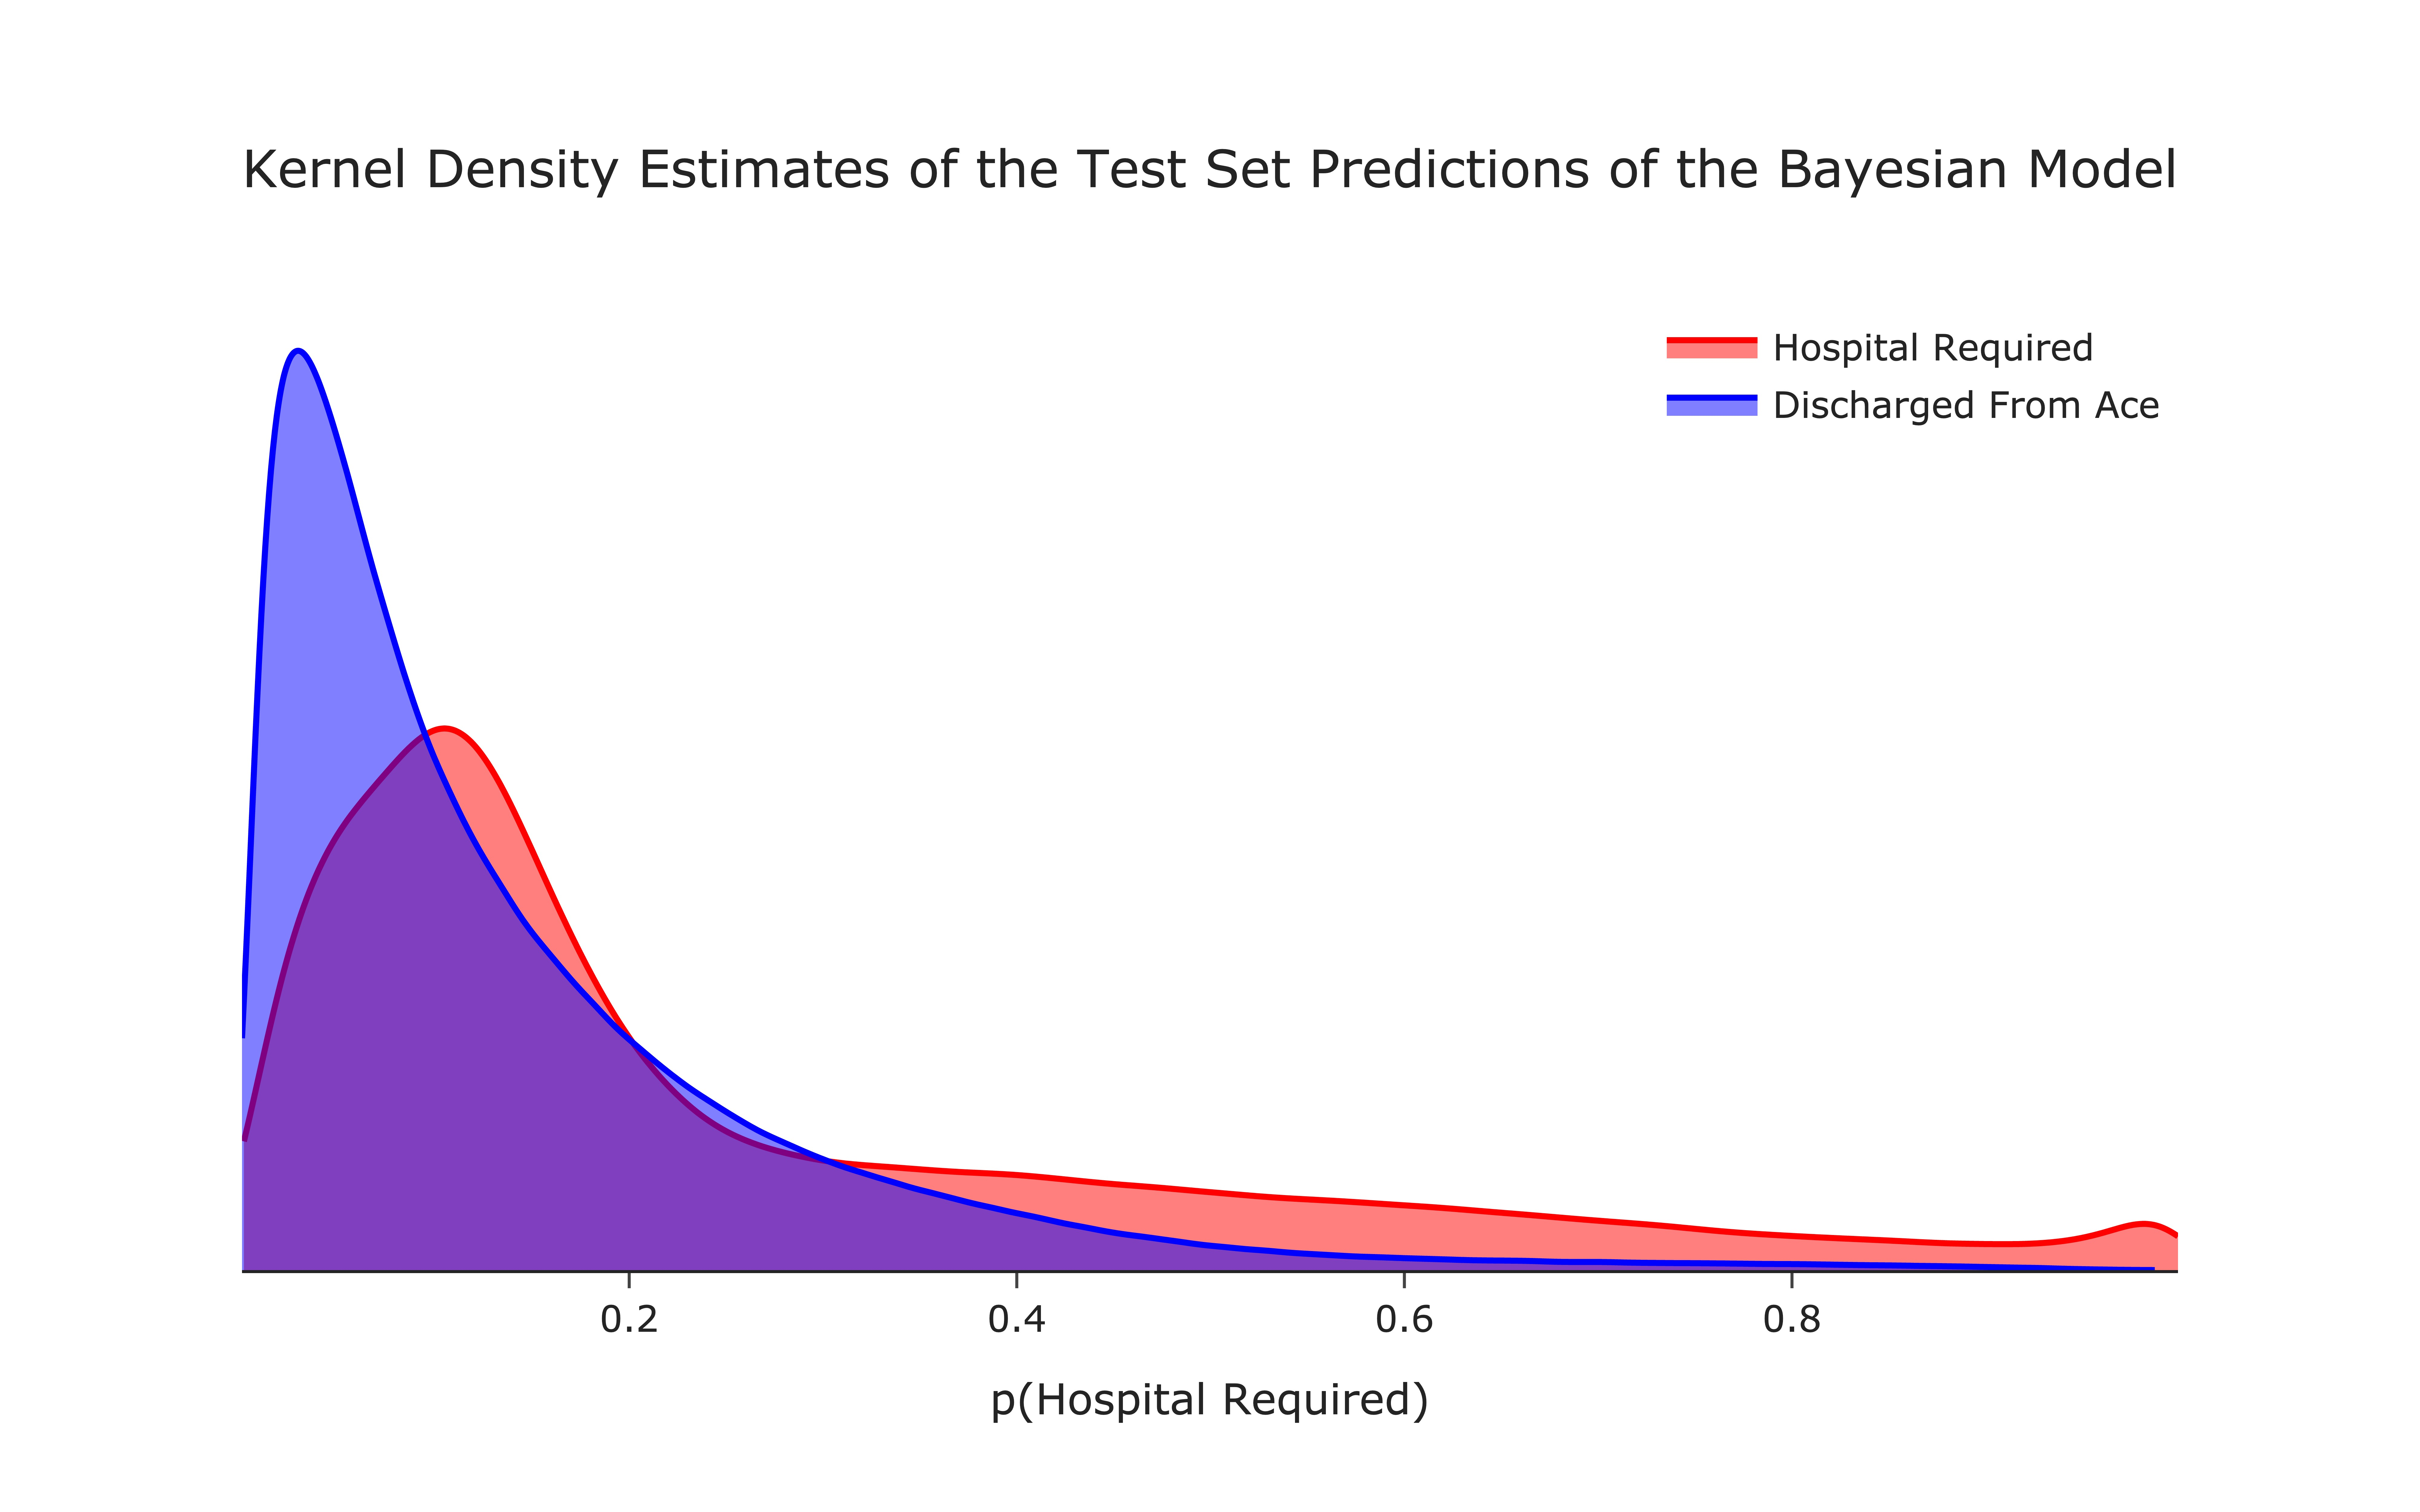
\includegraphics[width=1\textwidth]{test-pred-kdes}
    \caption[Kernel density estimates for Bayesian predictions]{Kernel density estimates for all the sample predictions from the Bayesian logistic regression model grouped by the true label - successfully treated by ACE or referred to hospital}
    \label{fig:test-pred-kdes}
\end{figure}

\begin{figure}[h]
    \centering
    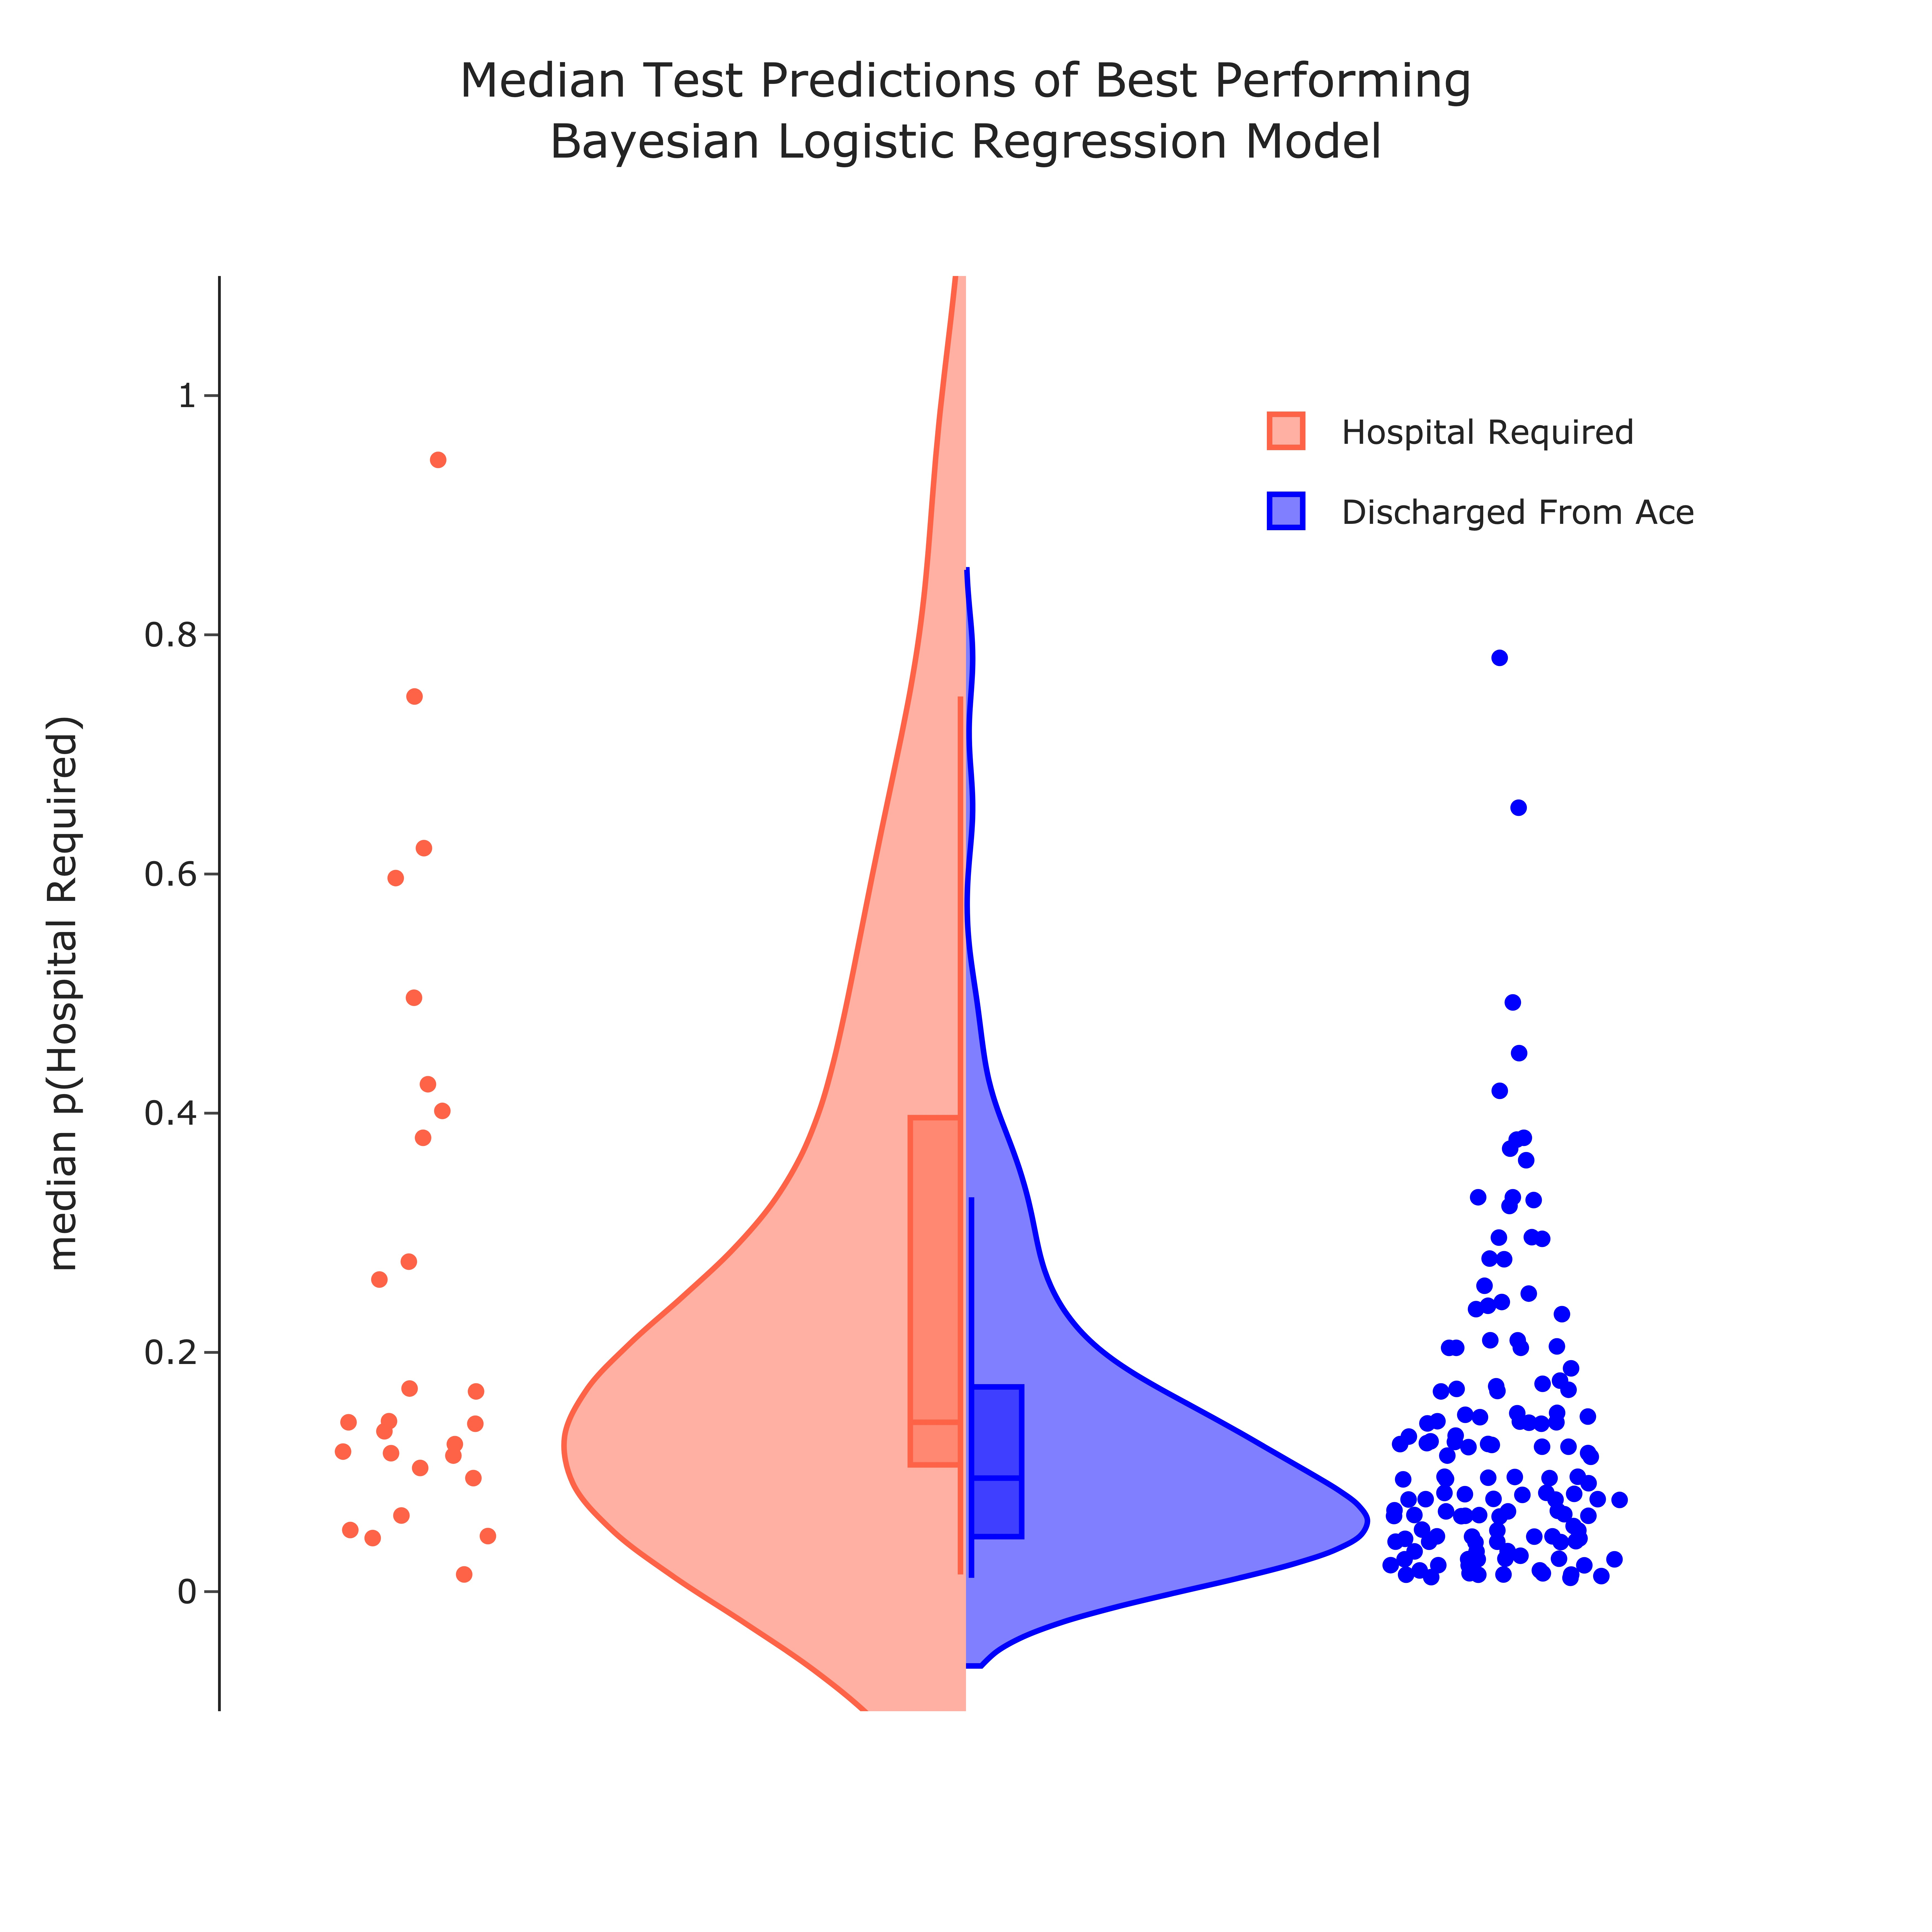
\includegraphics[width=0.7\textwidth]{median-preds}
    \caption[Predictions from Bayesian logistic regression model]{Combination Violin/Box/Scatter plot of the median predictions from the Bayesian logistic regression model, grouped by the true label. A trend of higher probabilities of hospitalisation can be seen among those examples that were referred to hospital, demonstrating the better performance of the Bayesian model over the models in \Cref{ch:classification-modelling}.}
    \label{fig:median-preds}
\end{figure}

\subsection{Reproducing results}\label{subsec:reproducing-results}

Code to reprodce the results of this experiment can be found in \textbf{\textit{models/pyMC3/bayes\_models.ipynb}}

\section{Conclusions}\label{sec:conclusions3}

The predictions of the Bayesian model clearly demonstrate that it is not possible to make confident predictions of hospitalisation from the ACE referral data. Though the predictions of the Bayesian model do show some separation between hospitalised patients and those discharged from ACE, it remains the case that the model assigned many of the hospitalised patients a low predicted risk and several patients that were successfully discharged a higher predicted risk. Generally, our model can either confidently predict successful treatment, or give a diffuse or uncertain range of hospitalisation probabilities. These findings support those in the initial data analysis (\Cref{ch:the-data}) and the frequentist classification modelling (\Cref{ch:classification-modelling}), and serve to reiterate that the ACE team are making good use of the referral data to identify patients at higher risk of hospitalisation.

Parameter estimates from the Bayesian logistic regression model clearly show a relationship between certain key features in the ACE referral data and treatment outcomes. Particularly effective were the features taken from the text notes that were added for this experiment. It is likely that the text features are more effective as they are not part of the ACE referral criteria, and thus they have not been specifically used when making the referral decisions that underpin each of the examples in the dataset. The parameter estimates of the final model indicate that the new text features interact with the other referral features to indicate hospitalisation risk. This highlights the promise of exploring other features from patient's medical histories that might prove to be powerful indicators of outcomes within the ACE service.

